\documentclass[11pt]{handout}
\usepackage{moreverb}
\usepackage{tabularx}
\usepackage{epsf}
\usepackage{epsfig}
\usepackage{fancyheadings}
\usepackage{fancybox}

\renewcommand{\coursetitle}{ECE 320}
\renewcommand{\handouttitle}{Chamberlin Filters}
\renewcommand{\handoutauthor}{Swaroop Appadwedula}
\renewcommand{\semestertitle}{Spring 2000}

\newcommand{\bea}{\begin{eqnarray}}
\newcommand{\eea}{\end{eqnarray}}

\setlength{\parindent}{5mm}
\begin{document}

\setlength{\baselineskip}{0.5cm}
\setlength{\parskip}{0.5cm}

\makeboxtitle
\vspace{0.3cm}

\section{Introduction}
Chamberlin filter topology is frequently used in music applications 
where very narrow-band low-pass filters are necessary.  Chamberlin 
implementations do not suffer from stability problems that arise 
in direct-form implementations of very narrow-band responses.  For more 
information about IIR/FIR filter design for DSPs, check out the 
Motorola Application Note \cite{Motorola}.

\section{Filter topology}
A Chamberlin filter is a simple 2-pole IIR filter with the transfer 
function
\begin{equation}
        H(z) = \frac{F_{c}^2 z^{-1}} 
        {1 - (2 - F_{c}Q_{c} - F_{c}^2) z^{-1} + (1-F_{c}Q_{c})z^{-2}}
\end{equation}
where $F_{c}$ determines the frequency where the filter peaks, and 
$Q_c = 1/Q$ determines the rolloff.  $Q$ is defined as the 
positive ratio of the center frequency to the bandwidth.  
A derivation of Chamberlin filters 
and more detailed explanation is given in \cite{Dattorro}.  
The topology of the filter is shown in Figure \ref{fig:chamberlin}.  
Note that the final feed-back stage puts a pole just inside the unit 
circle on the real axis.  For a response with smaller bandwidth, the 
pole should be moved closer to the unit circle, while making sure of 
stability.  Also, multiple second-order sections can be cascaded to 
yield a sharper rolloff.

\begin{figure}[htb]
   \begin{center}
      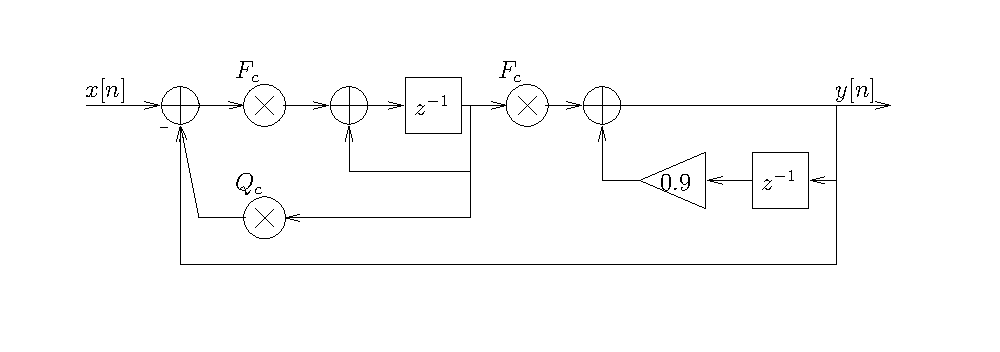
\epsfig{file=chamberlin.eps,width=13cm}
      \vspace*{0.5cm}
      \caption{Chamberlin filter topology}
      \label{fig:chamberlin}
   \end{center}
\end{figure}

Figures \ref{fig:chamberlinQc} and \ref{fig:chamberlinFc} show how 
the response of the filter varies with $Q_c$ and $F_c$.

\begin{figure}[htb]
   \begin{center}
      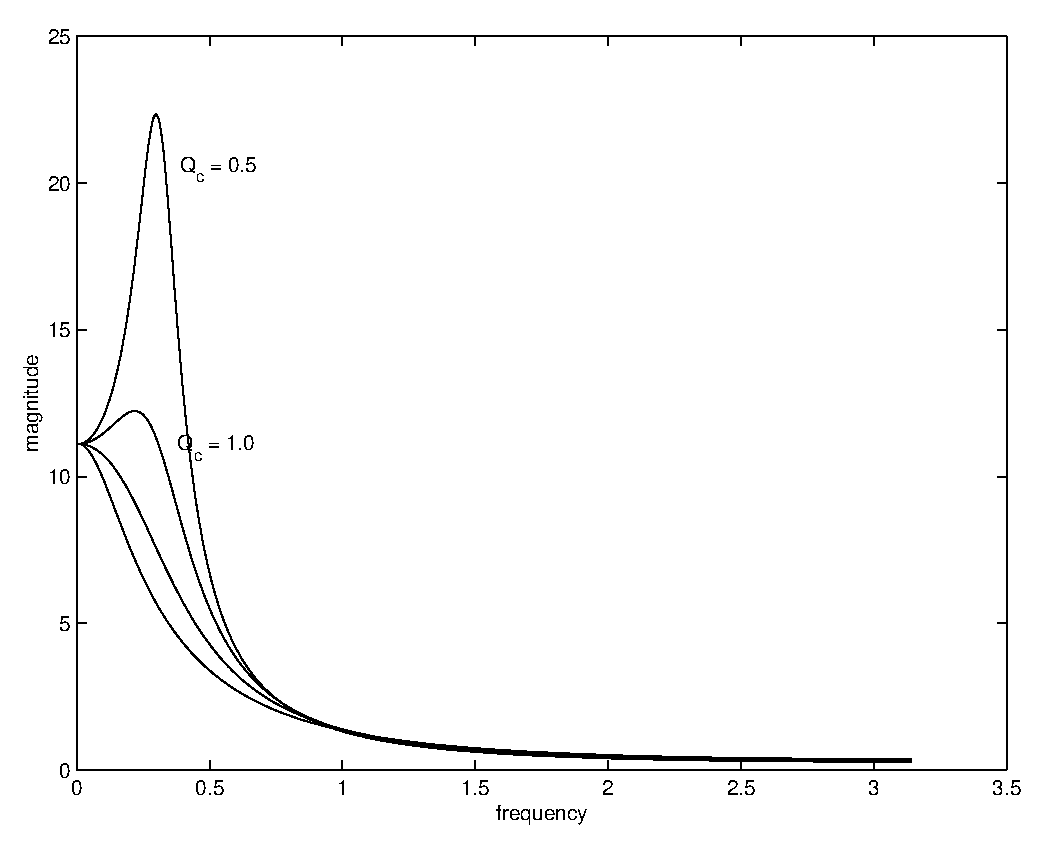
\epsfig{file=chamberlinQc.eps,width=11cm}
      \vspace*{0.5cm}
      \caption{Chamberlin filter responses for various $Q_c$ ($F_c=0.3$)}
      \label{fig:chamberlinQc}
   \end{center}
\end{figure}

\begin{figure}[htb]
   \begin{center}
      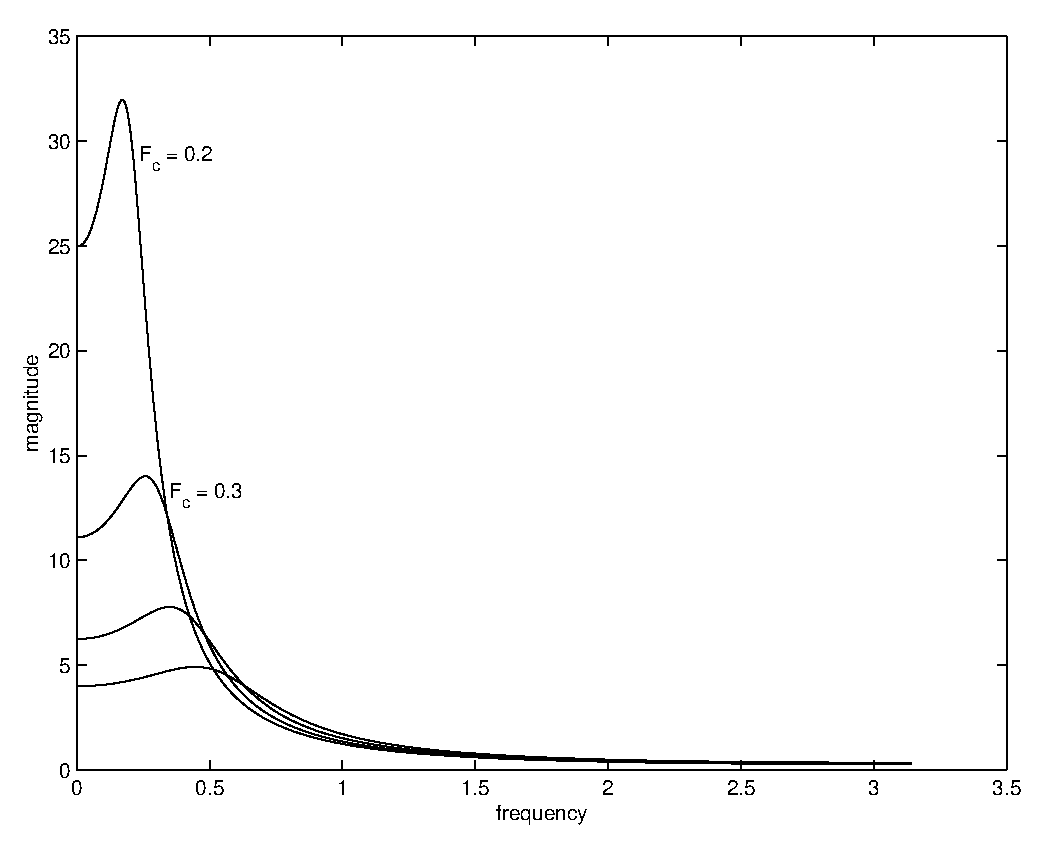
\epsfig{file=chamberlinFc.eps,width=11cm}
      \vspace*{0.5cm}
      \caption{Chamberlin filter responses for various $F_c$ ($Q_c=0.8333$)}
      \label{fig:chamberlinFc}
   \end{center}
\end{figure}

\small
\ifx\undefined\allcaps\def\allcaps#1{#1}\fi
\begin{thebibliography}{2}

\bibitem{Dattorro}
J. Dattotto, ``Effect Design Part 1: Reverberator and Other Filters,'' 
{\em Journal Audio Engineering Society}, vol.~45, pp.~660--684, Sept. 1997.

\bibitem{Motorola}
Motorola, ``Implementing IIR/FIR Filters with Motorola's DSP56000/SPS/DSP56001 
Digital Signal Processors,'' 
{\em http://www.mot.com/pub/sps/dsp/library/appnotes/apr7.pdf}.

\end{thebibliography}

\end{document}


